


\section{Performances of Transciphering with \coolName}
\label{sec:bench}


This section focuses on the performances of transciphering with \coolName. We first address the wrapping of a (\coolName) symmetric key as a compact set of TFHE ciphertexts for which we additionally introduce a trade-off between bandwidth and computation. Next, we explain how to manage different data representations to be able to fit with the input format of the server application. We then provide a detailed description of the homomorphic evaluation of \coolName. We finally give some implementation benchmarks and comparison to the state of the art.

\subsection{Key Wrapping and Bandwidth in TFHE Transciphering} \label{sec:key_wrapping}

Assume one wants to generate a fresh TFHE ciphertext vector $(c_1, \ldots, c_t)$ for a plaintext vector $(m_1, \ldots, m_t) \in \mathbb{Z}_p^t$, where $c_i = (a_{i,1}, \ldots, a_{i,n}, b_i)$, for every $i \in [1,t]$. Since the $a_{i,j}$'s are uniformly sampled at random over $\mathbb{Z}_q$, a folklore trick is to generate them pseudorandomly from a seed. We get the following compressed encryption procedure (where $\lambda$ denotes the security level in bits):
  
\begin{center}
\noindent\framebox{
\begin{minipage}{0.8\textwidth}
\underline{$\mathtt{CompressEncrypt}(s,m_1, \ldots, m_t)$}
	\vspace{-2mm}
	\begin{enumerate}
	\item Sample $\mathsf{seed} \gets \{0,1\}^\lambda$
	\smallskip
	\item Expand $((a_{i,j})_{1 \leq j \leq n})_{1 \leq i \leq t} \gets \mathsf{PRG}(\mathsf{seed})$
	\smallskip
	\item $\forall \:i \in [1,t]$: $b_i \gets \sum_{j=1}^n a_{i,j} \cdot s_j + \tilde{m}_i + e_i$ with $e_i \gets \chi_{\sigma}$
	\smallskip
	\item Return $(\mathsf{seed}, b_1, \ldots, b_t)$
\end{enumerate}
\end{minipage}}
\end{center}

\smallskip

Recovering standard TFHE ciphertexts $c_1$, \ldots, $c_t$ from the compressed form $(\mathsf{seed}, b_1, \ldots, b_t)$ is simply done by expanding the $a_{i,j}$'s from $\mathsf{seed}$. The size of the obtained compressed ciphertext vector is $\lambda + t \cdot \log_2(q)$ against $t \cdot (n+1) \cdot \log_2(q)$ for a standard TFHE encryption, meaning a compression by a factor about $(n+1)$. 

This compressed TFHE encryption method can be applied directly to transmit homomorphically encrypted data from the user to the server. Alternatively, it can be combined with transciphering to encrypt a symmetric key. The resulting bandwidth requirements and the corresponding plaintext-to-ciphertext expansion factor are summarized in Table~\ref{tab:formulas_bandwidth}, where they are further compared with the naive (uncompressed) TFHE encryption. In particular, for \coolName, a wrapped key is of size $\lambda + (|\mathcal K| + |\mathcal W|) \cdot \log_2(q)$, (which in our case gives 784 bytes) for a security of $\lambda = 128$ bits (target security of \coolName), the standard choice of $q= 2^{64}$ (which we use in our implementation) and $|\mathcal K| + |\mathcal W| = 96$ per the specification of \coolName (see Section~\ref{sec:description}). This fixed cost is hence very quickly amortized while the amount of data to encrypt grows.
Moreover, this approach can be applied to the server keys as well, which are actually encryptions of the secret key's bits. We took this optimization into account in our estimations of the server key sizes in Table \ref{tab:server_key_size}. 

\paragraph{Compressing further.}

We introduce hereafter a tweak to compress a TFHE encryption further than the folklore compression. By definition of the TFHE encryption process, the least significant bits of the body $b_i = \sum_{j=1}^n a_{i,j} \cdot s_j + \tilde{m}_i + e_i$ are randomized by the error $e_i$ and can hence be discarded without loss of information. We can thus tweak the above compressed encryption process by returning $(\mathsf{seed}, \mathrm{Tr}_\ell(b_1), \ldots, \mathrm{Tr}_\ell(b_t))$ where $\mathrm{Tr}_\ell(\cdot)$ denotes the truncation of the $\ell$ least significant bits. To decompress such ciphertexts, besides pseudorandomly generating the masks from the seed, one just needs to pad the truncated bodies with $\ell$ bits to $0$. By the randomness of the mask, the effect of this truncation plus $0$-padding is to add a uniform random error of $\ell$ bits to the body, namely an error of standard deviation: 
$$\sigma_0^2  = \frac{(2^\ell - 1)^2}{12} \approx \frac{2^{2\ell}}{12} \approx 0.08 \cdot 2^{2\ell} ~.$$

\noindent This optimization comes in two flavors:
\begin{enumerate}
	\item \emph{The ``free'' variant.} The number of truncated bits $\ell$ is selected to have a small impact on the noise distribution. For instance in \coolName, the noise of the fresh ciphertexts is summed with the noise coming from the FSM. Thus, we can compute $\ell$ to keep $\sigma^2_{\mathcal W} < \sigma^2_{\text{PBS}}$. Our experiments shows $\sigma^2_{\text{PBS}} = 2^{52}$, so running the numbers we find that we can truncate up to $\ell=19$ bits, allowing to reduce the volume of the TFHE ciphertexts to send by a factor $1 - \frac{19}{64} \approx 0.7$.
	
	\smallskip
	
	\item \emph{The communication-computation trade-off.} In this variant, one selects a high value of $\ell$. The truncated body should at least contain $\log_2(p)$ bits to keep the plaintext information, plus a margin of a few bits in order to remain bootstrappable. Denoting this margin $\delta$, the truncated body should be of at least $\log_2(p) + \delta$ bits and $\ell$ can be up to $\log_2(q) - (\log_2(p)+\delta)$. Taking the maximum level of truncation, inducing the maximum level of bootstrappable noise, implies some adaptation of the underlying homomorphic computation. Specifically, it should start with applying a noise-reduction bootstrapping to the decompressed ciphertexts before performing the original evaluation. We hence obtain a trade-off with reduced bandwidth against additional bootstrappings.
\end{enumerate}

In the context of transciphering with \coolName, the trade-off provided by the second option gives rise to an initialization procedure which consists in decompressing and bootstrapping the wrapped key. 




\begin{table}[t!]
	\centering
        \caption{Bandwidth of homomorphic ciphertexts (in bits).}
        % The total bandwidth is the fixed cost + $t$ times the cost per message to encrypt $(m_1, \ldots, m_t)\in \mathbb{Z}_p^t$.
	\label{tab:formulas_bandwidth}
        {
          \renewcommand{\arraystretch}{1.1}
          \footnotesize
          \scalebox{0.9}{
            \begin{tabular}{|l|*{3}{>{\centering\arraybackslash}p{3.5cm}|}}
              \hline
              \textbf{Approach used} & \textbf{Naive} & \textbf{Compressed} & \textbf{\coolName} \\
              \hline
              Fixed cost & 0 & $\lambda$ & $\lambda + (|\mathcal{K}|+|\mathcal{W}|) \cdot \log_2(q)$ \\
              \hline
              Per message in $\mathbb{Z}_p$ & $(n+1) \cdot \log_2(q)$ & $\log_2(q)$ & $\log_2(p)$ \\
              \hline
              Expansion factor~ & $(n+1) \cdot {\log_2(q)}/{\log_2(p)}$ & ${\log_2(q)}/{\log_2(p)}$ & 1 \\
              \hline
            \end{tabular}}
        }
	
\end{table}



\subsection{Transciphering vs. Data Representation}
\label{sec:data_representation}

Managing data representation is a common challenge when working with TFHE. Since this scheme is only efficient at very low precision, an abstraction layer is required to construct practical data types (e.g., 8-, 32-, or 64-bit integers) from smaller encrypted chunks. Common constructions include radix-based decompositions and Chinese Remainder Theorem (CRT) representations, leading to different efficiency trade-offs. Carry propagation in radix-based representations is notoriously slow due to the large number of required bootstrappings, while CRT representations impose constraints on feasible operations. These constructions have been studied in~\cite{JC:BBBCLOT23}. 

As a result, there is no universal representation that is optimal for all homomorphic operations. Thankfully, the representation of data in the transciphering algorithm can be chosen independently of that of the homomorphic application running on the server. If the representation in $\mathbb Z_p$ does not suit the application, the server can convert the ciphertexts to the desired representation before running the application. %Such a conversion can be either applied to the TFHE ciphertexts obtained by the server after transciphering, or directly on the keystream (in this case, the symmetric ciphertexts are encoded directly in the desired representation, and the encryption/decryption operation is performed in the corresponding space). In both cases, it simply requires a bootstrapping for each element of $\mathbb Z_p$. 
We stress that this additional step of conversion would be necessary for any transciphering algorithm, as the data format desired in output of transciphering is completely application-dependent.

	
As a concrete example, assume that the data to be encrypted (i.e., the input to the homomorphic computation) consists of elements from $\mathbb{Z}_{16}$. The overall transciphering process unfolds as follows. On the client side, the plaintext is first embedded from $\mathbb{Z}_{16}$ into $\mathbb{Z}_{17}$ before being encrypted using \coolName. On the server side, the keystream is homomorphically generated and then used to homomorphically decrypt the ciphertext. This results in a TFHE encryption of the original plaintext, now embedded in $\mathbb{Z}_{17}$, meaning that the plaintext space for the TFHE encryption is $\mathbb{Z}_{17}$. A programmable bootstrapping (PBS) operation is then applied to switch the plaintext space from $\mathbb{Z}_{17}$ back to $\mathbb{Z}_{16}$.

In terms of computation, this process adds one PBS per $\mathbb{Z}_{16}$-element of the original plaintext, in addition to the four PBS per element required for keystream generation with \coolName. Moreover, embedding $\mathbb{Z}_{16}$ into $\mathbb{Z}_{17}$ increases the size of the encrypted data by a factor of $1 + 1/16 = 1.0625$.

This approach can be generalized to address other plaintext representations. In particular, for larger chunks of bits, the bootstrapping operation would allow to merge several elements of $\mathbb{Z}_{16}$ (embedded into $\mathbb{Z}_{17}$) into one element of $\mathbb{Z}_{2^\ell}$ with $\ell > 4$. On the other hand, one may split an element of $\mathbb{Z}_{16}$ (or its $\mathbb{Z}_{17}$ embedding) into 4 elements of $\mathbb{Z}_{2}$ using a PBS with multiple look-up tables (``PBSmanyLUT'') as proposed in~\cite{AC:CLOT21}.



	
\subsection{Detailed Homomorphic Implementations}
\label{sec:detailed_implementation}

In the following, we provide a more detailed way of how we implemented the homomorphic version of \coolName.

\paragraph{Homomorphic evaluation of LFSRs.}
The \coolName design involves two LFSRs operating on elements of $\F_{17}$. The standard way to implement an LFSR is to evaluate the linear feedback function on the state at each clock cycle, thus producing a new element that enters the state, while the state is shifted to output an element. 

We suggest the \emph{silent LFSR} approach for the homomorphic evaluation of LFSRs. In this approach, the encrypted LFSR state is immutable to avoid any noise growth in the underlying ciphertexts (hence keeping the LFSR ``silent''). We use the fact that every output element of the LFSR can be expressed as a linear combination of the initial state. So, at each clock cycle, we compute \emph{in the clear} the coefficients of this linear combination and homomorphically evaluate it on the immutable encrypted state. This process is depicted in Algorithm~\ref{alg:lsfr}.


\begin{algorithm}[t!]
    \caption{\texttt{LFSR.clock} - Produce a pseudo random element of the state. \label{alg:lsfr}}
    
    \KwIn{
        $\left\{
        \begin{aligned}
            &\ell: \text{ Size of the state of the LFSR.} \\
            &(u_1, \dots, u_\ell): \text{ Encrypted initial state of the LFSR.} \\
            &(\lambda_1^{(0)}, \dots, \lambda_\ell^{(0)}): \text{ Coefficients of retroaction in the definition of the LFSR.} \\
            &(\lambda_1^{(i)}, \dots, \lambda_\ell^{(i)}): \text{ Previous coefficients used in the linear combination.}
        \end{aligned}
        \right.$
    }

    \KwResult{
        $\left\{
        \begin{aligned}
            &o^{(i)}: \text{ Encryption of the $i$-th pseudorandom element of $\F_{17}$.} \\
            &(\lambda_1^{(i+1)}, \dots, \lambda_\ell^{(i+1)}): \text{ Updated coefficients of the linear combination.}
        \end{aligned}
        \right.$
    }

    % Add vertical space and horizontal line
    \vspace{0.5em} % adjust the space as needed
    \hrule
    \vspace{0.5em} % adjust the space as needed

    $o^{(i)} \gets 0$

    \Comment{Evaluation of the linear combination}
    \For{$k \in \{1, \dots, \ell\}$}{
        $o^{(i)} \gets \texttt{SumTFHE}(o^{(i)}, \texttt{ClearMultTFHE}(u_k, \lambda_k^{(i)}))$
    }
    \Comment{Update of the next coefficients}
    \For{$k \in \{2, \dots, \ell\}$}{
        $\lambda_k^{(i+1)} \gets \lambda_{k-1}^{(i)} + \lambda_\ell^{(i)} \cdot \lambda_k^{(0)}$
    }
    $\lambda_1^{(i+1)} \gets \lambda_\ell^{(i)} \cdot \lambda_1^{(0)}$
    
    \Return{$o^{(i)}$}
    
\end{algorithm}




\paragraph{Homomorphic evaluation of} \coolName. The complete homomorphic evaluation of a round of on clock cycle of \coolName is depicted in Algorithm~\ref{alg:transistor}, using $\pseudoKS.\texttt{clock}$ and $\whitening.\texttt{clock}$ as subroutines (i.e., Algorithm~\ref{alg:lsfr} evaluated on the key schedule and whitening LFSRs). The most computation intensive part of the algorithm is by far the evaluation of the PBS in $\subWords$ which can be fully parallelized to reduce the latency.


 \begin{algorithm}[t!]
    \caption{\texttt{Transistor.clock} - Produce $r$ encypted elements of the key stream}
    \label{alg:transistor}
    
 
    \KwIn{
        $\left\{
        \begin{aligned}
        	&\mathcal K: \text{the LFSR used for the pseudo-keyschedule and its state (cf Algorithm \ref{alg:lsfr}).}\\
            &\mathcal W: \text{the LFSR used for the whitening.}\\	
            &X = \left ( \begin{array}{ccc}
            x_{1,1} & \dots & x_{1,\sqrt{m}}\\
            \dots & \dots & \dots\\
            x_{\sqrt{m},1} & \dots & x_{\sqrt{m},\sqrt{m}}\\
            \end{array} \right ): \text{ Encrypted state of the FSM} \\
        \end{aligned}
        \right.$
    }

    \KwResult{
        $\left\{
        \begin{aligned}
            &Y = (y_1, \dots, y_r): \text{ Encryption of $r$ elements of the  key stream } \\
        \end{aligned}
        \right.$
    }

    % Add vertical space and horizontal line
    \vspace{0.5em} % adjust the space as needed
    \hrule
    \vspace{0.5em} % adjust the space as needed

    \Comment{Compute the pseudo-key schedule and adds it to the FSM}
    \For{$i \in [1, \sqrt m]$}{
        \For{$j \in [1, \sqrt m]$}{
            $k_{i,j} \gets \pseudoKS.\texttt{clock}()$\\
            $x_{i,j} \gets \texttt{SumTFHE}(x_{ij}, k_{i,j})$\\
        }
    }
    \Comment{Compute $\subWords$ with a layer of PBS}
    \For{$i \in [1, \sqrt m]$}{
        \For{$j \in [1, \sqrt m]$}{        
            $x_{i,j} \gets \texttt{PBS\_TFHE}(x_{i,j}, S)$\\
        }
    }
    \Comment{Extract the output bits and whiten them}
    $(y_1, \dots, y_r) \gets \phi(X)$\\
    \For{$i \in [1, r]$}{
        $w_i \gets \whitening.\texttt{clock}()$\\
        $y_i \gets \texttt{SumTFHE}(y_i, w_i)$\\
    }
    \Comment{Compute $\shiftRows$, (same as in clear)}
    $X \gets \shiftR(X)$

    \Comment{Compute MixColumns}
    \For{$i \in [1, \sqrt m]$}{
        \For{$j \in [1, \sqrt m]$}{
            $z_{i, j} \gets 0$\\
            \For{$k \in [1, \sqrt m]$}{
                $z_{i, j} \gets \texttt{SumTFHE}(z_{i, j}, \texttt{ClearMultTFHE}(x_{k, j}, MC_{i, k}))$\\
            }
        }
    }

    \Return{$Y$}

\end{algorithm}






\subsection{TFHE Parameters} 
\label{sec:tfhe-parameters}
\TODO{Trouver une solution pour harmoniser avec Orpheus (mais écrire le chapitre en question d'abord)}

\ifeprint
\else
	The details of the homomorphic implementation of \coolName{} are given in the full version~\cite{EPRINT:BBBBCL25}. In short, the LFSRs are clocked in a silent way (see Section \ref{sec:rationale-controllin-noise}), and the implementation of the rest of the algorithm is straightforward using the basics operations provided by the TFHE scheme (see Section~\ref{sec:preliminaries}). 
\fi

We discuss hereafter the selection of the different TFHE parameters involved in the homomorphic implementation of \coolName. Here is the list of the different parameters to be considered:
\begin{itemize}
	\item $q$: the modulo used for the ciphertexts,
	\item $n_{\text{short}}$: the dimension of the LWE ciphertexts used within the PBS algorithm,
	\item $k$: the dimension of GLWE ciphertexts,
	\item $N$: the degree of the polynomials in GLWE ciphertexts,
	\item $n_{\text{long}} = k \cdot N$: the dimension of the LWE ciphertexts extracted from GLWE ciphertexts,
	\item $\sigma_{\text{short}}, \sigma_{\text{long}}$: the standard deviation of the Gaussian distribution of fresh noise in the ciphertexts of dimension respectively $n_{\text{short}}$ and  $n_{\text{long}}$,
	\item $B_{KS}$ and $B_{BR}$: the bases used in the gadget decompositions occurring in respectively the \textsf{Keyswitching} and the \textsf{BlindRotate} phases,
	\item $\ell_{KS}$ and $\ell_{BR}$: the levels of those decompositions.
\end{itemize}

Throughout the homomorphic evaluation of \coolName, the manipulated ciphertexts can be of three different types: LWE ciphertexts of dimension $n_{\text{short}}$, LWE ciphertexts of dimension $n_{\text{long}}$, or GLWE ciphertexts of dimension $k$ and polynomial degree $N$. \ifeprint{
	Figure \ref{fig:structure_fhe} shows the ciphertext format at the different steps of the homomorphic evaluation.
	
	\begin{figure}[t!]
  \centering
    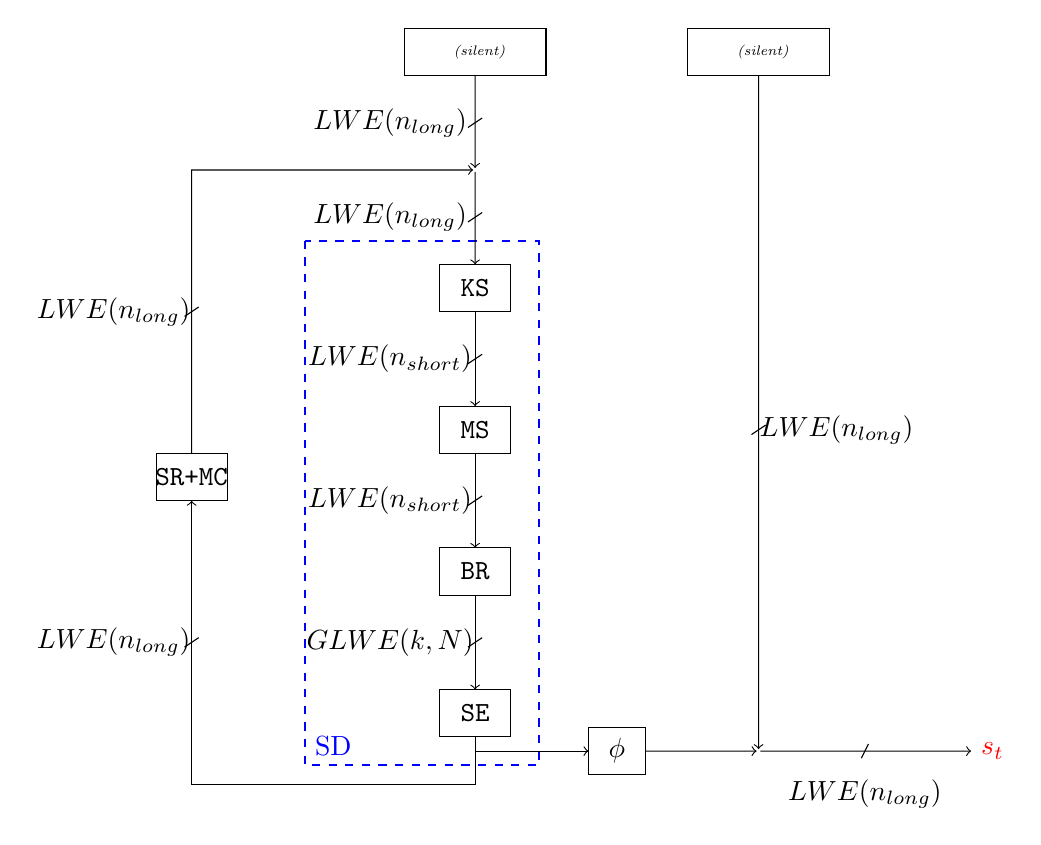
\begin{tikzpicture}[xscale=0.9,yscale=0.6]
 
    %LSFRs
    \draw[] (0, 0) rectangle (2, 1) node[pos=0.5]{$\pseudoKS$ {\tiny \emph{(silent)}}} ;
    \draw[] (4, 0) rectangle (6, 1) node[pos=0.5]{$\whitening$ {\tiny \emph{(silent)}}} ;
    \draw (1, -2) node[inner sep=0pt](addm){$\boxplus$} ;
    \draw[->] (1, 0) -- (addm);

    % FSM
    \draw[] (0.5, -4) rectangle (1.5, -5) node[pos=0.5,color=black](ks){$\texttt{KS}$} ;
    \draw[] (0.5, -7) rectangle (1.5, -8) node[pos=0.5,color=black](ms){$\texttt{MS}$} ;
    \draw[] (0.5, -10) rectangle (1.5, -11) node[pos=0.5,color=black](br){$\texttt{BR}$} ;
    \draw[] (0.5, -13) rectangle (1.5, -14) node[pos=0.5,color=black](se){$\texttt{SE}$} ;
    \draw[] (-3.5, -8) rectangle (-2.5, -9) node[pos=0.5,color=black](srmc){$\texttt{SR+MC}$} ;

    % Draw dashed blue box for SB
    \draw[dashed, blue, thick] (-1.4, -3.5) rectangle (1.9, -14.6);
    \node[blue] at (-1, -14.2) {SD}; % Label for the box

    % FSM connections
    \draw[->] (addm) -- (1, -4);
    \draw[->] (1, -5) -- (1, -7);
    \draw[->] (1, -8) -- (1, -10);
    \draw[->] (1, -11) -- (1, -13);
    \draw[->] (1,-14) -- (1, -15) -- (-3, -15) -- (-3, -9);
    \draw[->] (-3, -8) -- (-3, -2) -- (addm);

    % Extraction
    \draw (5, -14.3) node[inner sep=0pt](addr){$\boxplus$} ;
    \draw[] (2.6, -13.8) rectangle (3.4, -14.8) node[pos=0.5,color=black]{$\phi$} ;

    \draw[->] (1, -14.3) -- (2.6, -14.3);
    \draw[->] (3.4, -14.3) -- (addr);
    \draw[->] (5, 0) -- (addr);
    \draw[->] (addr) -- (8, -14.3);
    \draw[color=red] (8.3, -14.3) node(s){$s_t$} ;



    % Wire type
    \draw (0.9, -1.1) -- (1.1, -0.9) ;
    \draw (-0.2, -1) node{$LWE(n_{\text{long}})$} ;
    \draw (0.9, -3.1) -- (1.1, -2.9) ;
    \draw (-0.2, -3) node{$LWE(n_{\text{long}})$} ;
    \draw (0.9, -6.1) -- (1.1, -5.9) ;
    \draw (-0.2, -6) node{$LWE(n_{\text{short}})$} ;
    \draw (0.9, -9.1) -- (1.1, -8.9) ;
    \draw (-0.2, -9) node{$LWE(n_{\text{short}})$} ;
    \draw (0.9, -12.1) -- (1.1, -11.9) ;
    \draw (-0.2, -12) node{$GLWE(k, N)$} ;
    \draw (-3.1, -12.1) -- (-2.9, -11.9) ;
    \draw (-4.1, -12) node{$LWE(n_{\text{long}})$} ;
    \draw (-3.1, -5.1) -- (-2.9, -4.9) ;
    \draw (-4.1, -5) node{$LWE(n_{\text{long}})$} ;
    \draw (4.9, -7.6) -- (5.1, -7.4) ;
    \draw (6.1, -7.5) node{$LWE(n_{\text{long}})$} ;
    \draw (6.45, -14.45) -- (6.55, -14.15) ;
    \draw (6.5, -15.2) node{$LWE(n_{\text{long}})$} ;

    \end{tikzpicture}
  \vspace{1em}
  \hfill~
  \caption{\label{fig:structure_fhe} Types and shapes of ciphertexts in homomorphic \coolName. The $\subWords$ is broken down into its elementary components}
\end{figure}


% Leo: ce qui suit est pour qu'emacs compile bien l'article, pas touche !
%%% Local Variables:
%%% mode: latex
%%% ispell-local-dictionary: "english"
%%% TeX-master: "../main"
%%% End:




}
\else %{Appendix~\ref{sec:schema_structure_fhe} shows the ciphertext format at the different steps of the homomorphic evaluation.

\fi

\paragraph{Optimization of the TFHE parameters.}
To generate a set of parameters, we use the method developed in~\cite{JC:BBBCLOT23}. Given the negligible noise contribution from the LFSRs, the FSM can be modeled using the \emph{atomic pattern} introduced in~\cite{JC:BBBCLOT23} (specifically the instance referred to as $\mathcal{A}^{(\text{CJP21})}$), which is a pattern of homomorphic operators taking a set of ciphertexts in input, computing linear combinations of those ciphertexts and applying a programmable bootstrapping to each of them. The FSM round in \coolName which composes a multiplication by a constant matrix ($\mixColumns$), followed by a bootstrapping step ($\subWords$) is precisely an instance of such an atomic pattern. The framework proposed in~\cite{JC:BBBCLOT23} generates parameters that guarantee a specified security level $\lambda$ for the LWE encryption and target error probability $p_{\text{err}}$, while optimizing the PBS to be as fast as possible. 
\ifeprint{
		Table \ref{tab:parameters} shows the parameters used for our experiments, all ensuring 128 bits of security. The obtained security levels $\lambda_{\text{short}}$ et $\lambda_{\text{long}}$ have been estimated using the \texttt{lattice estimator}~\cite{lattice-estimator}.
		
		\begin{table}[t!]
		\centering
		\caption{TFHE Parameters used in our experiments}.
		\label{tab:parameters}
		\renewcommand{\arraystretch}{1.3}  % Adjust row spacing
		\scalebox{1}{
			\begin{tabular}{|c||*{12}{>{\centering\arraybackslash}p{0.8cm}|}}
				\hline
				$p_{\text{err}}$ & $q$ & $n_{\text{short}}$ & $k$ & $N$ & $\sigma_{\text{short}}$ & $\sigma_{\text{long}}$ & $B_{BR}$ & $\ell_{\text{BR}}$ & $B_{KS}$ & $\ell_{\text{KS}}$ & $\lambda_{\text{short}}$ & $\lambda_{\text{long}}$\\
				\hline
				$2^{-40}$ & $2^{64}$ & 788 & 2 & 1024 & $2^{47}$ & $2^{14}$ & $2^{23}$ & 1 & $2^4$ & 3 & 131.8 & 128.9\\
				\hline
				$2^{-128}$ & $2^{64}$ & 774 & 1 & 2048 & $2^{47}$ & $2^{14}$ & $2^{23}$ & 1 & $2^3$ & 5 & 131.8 & 128.9\\
				\hline
		\end{tabular}
		}
	\end{table}
}
\else{
    The parameters we use in our implementation for the two different error probabilities $p_{\text{err}}$: $2^{-40}$ and $2^{-128}$ are specified in the full version~\cite{EPRINT:BBBBCL25}.
}
\fi


\paragraph{Encryption security.} 
The security level (in bits) of the LWE ciphertexts is a function of the modulus $q$, the dimension $n$ and the noise standard deviation $\sigma$. While no explicit formula exists for this function, the \emph{lattice estimator} tool allows to produce an estimation of this function by simulating the main attacks of the literature~\cite{lattice-estimator}, which we denote $\mathcal{O}$ (for \emph{security oracle}). The selected TFHE parameters are constrained to satisfy $\mathcal{O}(q,n,\sigma) \geq \lambda$ for both $(q,n,\sigma) = (q,n_{\text{short}},\sigma_{\text{short}})$ and $(q,n,\sigma) = (q,n_{\text{long}},\sigma_{\text{long}})$.



\paragraph{Correctness of the PBS.} To compute the error probability $p_{\text{err}}$, we have to evaluate the variances occurring inside the programmable bootstrapping of the $\subWords$ layer\ifeprint. We provide such an analysis in Appendix \ref{sec:pbs_variance_analysis}. \else (see full version~\cite{EPRINT:BBBBCL25}).\fi
\TODO{Dans l'appendix, il y a l'analyse du bruit dans le PBS. A merger avec ORPHEUS}
In the following, we denote the maximum error probability of the bootstrapping by $p_{\text{err}} := 2^{-\kappa}$. We aim to choose parameters such that the PBS outputs a correct ciphertext with probability at least $1-p_{\text{err}}$. This translates to the following constraint:
$$\sigma^2_{\text{in-}\textsf{BR}} \leq  C(\kappa) \cdot \left(\frac1{4p}\right)^2 ~~~\text{with}~~~C(\kappa) := \left(\frac{1}{\sqrt{2} \cdot \mathsf{erfc}^{-1}(2^{-\kappa})}\right)^2 ~.$$
Under the Gaussian assumption, the noise in input of the \textsf{BlindRotate} is lower than $\mathsf{erfc}^{-1}(2^{-\kappa}) \cdot \sqrt{\sigma^2_{\text{in-}\textsf{BR}}}$ with probability $1-2^{-\kappa}$. The above constraint thus implies that, with probability $1-2^{-\kappa}$, the noise is lower than $1/{4p}$ which ensures the correctness of the PBS. 

As $|\mathcal W| \leq |\mathcal K|$, we can check that we always have $\sigma^2_{\text{out}} \leq \sigma^2_{\text{in-}\textsf{PBS}}$ which implies that the output is always bootstrappable with correctness probability at least $1-p_{\text{err}}$ in the subsequent bootstrapping.


\subsection{Performances} \label{sec:performances}

We provide hereafter some benchmarks of our implementation of \coolName for two sets of parameters tailored for two different error probabilities. We first consider $\perr = 2^{-40}$, which is a common choice in the literature to benchmark homomorphic implementations. Our results for this error probability allow a fair comparison with the state of the art. While such an error probability theoretically allows transciphering to be error-free with a large amount of data with good probability, some recent works have shown that non-negligible error probabilities could be exploited by an adversary in some contexts~\cite{EPRINT:CSBB24,EPRINT:CCPSS24}. Thus, we also provide another set of parameters and associated benchmark for $\perr =  2^{-128}$.

Our implementation relies on a customized version of \texttt{tfhe-rs}~\cite{tfhe-rs} which has been adapted to support odd $p$ (size of the plaintext space) as described in Chapter \ref{chap:p_encodings}. \TODO{Trouver où mettre l'adaptation de la lib dans le manuscrit et le référencer dans chaque partie impléméntation}. The experiments were carried on a processor 12th Gen Intel(R) Core(TM) i5-1245U with 4.4 GHz. Table \ref{tab:perfs} summarizes the obtained timings for the two sets of parameters. The throughput is computed assuming that $\log_2(17)$ bits are encoded on one element of $\F_{17}$. Encoding 4 bits on each element would scale the throughput by a factor $4/\log_2(17) \approx 0.98$.

\begin{table}[t!]
	\centering
		\caption{Performances of our two instances of \coolName.}
	\label{tab:perfs}
	\renewcommand{\arraystretch}{1.2}  % Adjust row spacing
	\begin{tabular}{|c||*{3}{>{\centering\arraybackslash}p{3cm}|}}
		\hline
		~~$p_{\text{err}}$~~ & Time for one PBS & Latency (one round) & Throughput\\
		\hline
		$2^{-40}$ & 11.9 ms & 195 ms & 83.84 bits/s\\
		\hline
		$2^{-128}$ & 15.28 ms & 251 ms & 65.10 bits/s\\
		\hline
	\end{tabular}
\end{table}



Although our current implementation does not leverage the inherent parallelism of \coolName, it is important to note that it can be easily parallelized across 16 threads. Specifically, during the $\subWords$ steps, which dominate the overall runtime, the 16 PBS operations can be executed concurrently. This parallelization would result in nearly a 16-fold reduction in total execution time.

Without taking into account the server key\ifeprint(whose sizes are shown in Table \ref{tab:server_key_size})\fi, and using compressed encryption (Section \ref{sec:key_wrapping}),  transciphering 1 KB of plain data requires 1.78 KB of data to be sent, instead of 64 KB. For larger amounts of message, the volume of the encrypted symmetric key becomes negligible with respect to the message: for 1 MB of plain data, we use 1.0008 MB, and for 1 GB, this goes down to 1.000001 GB. The two sets of parameters yield the same bandwidth consumption, but not the same running time as shown in Table \ref{tab:perfs}.



By applying the ``free truncation optimization" introduced in Section \ref{sec:truncature}, we can reduce the volume of the encrypted symmetric key by a factor~0.7. This is particularly useful when transciphering a small volume of data (the volume of the encrypted key being preponderant). For example, to transcipher 1 KB of data, using this technique decreases the volume from 1.78~KB to 1.54~KB. 

In Table \ref{tab:server_key_size} we provide the sizes for the server keys, namely the \emph{key-switching key} ($\KSK$) and the \emph{bootstrapping key} ($\BSK$) while using the ciphertext compression technique described in Section~\ref{sec:key_wrapping}. Those keys are only generated and communicated to the server once (during some user enrollment step).

\begin{table}[t!]
  \centering
  \caption{Size of the server keys for the two considered sets of parameters. 
    % This is agnostic to the volume of message sent. 
    \label{tab:server_key_size}}
  
  \renewcommand{\arraystretch}{1.2}  % Adjust row spacing
  \scalebox{0.9}{
    \begin{tabular}{|c||*{3}{>{\centering\arraybackslash}p{4cm}|}}
      \hline
      & Theoretical sizes & Sizes for $p_{\text{err}} = 2^{-40}$ & Sizes for $p_{\text{err}} = 2^{-128}$ \\
      \hline
      ~KSK~ &  $n_{\text{long}}\cdot l_{\text{KS}} \cdot \log_2 q $ & 49 KB & 82 KB  \\
      \hline
      ~BSK~ &  $n_{\text{short}} \cdot l_{\text{BS}} \cdot \log_2 q \cdot N \cdot (k+1)$ & 6.5 MB & 12.7 MB  \\
      \hline
    \end{tabular}
}
\end{table}




\subsection{Comparisons to the State of the Art}
\label{sec:perfs_soa}	

\subsubsection{Comparisons with other TFHE-friendly ciphers.} 
%In Section \ref{sec:soa}, we provided an overview of the recent landscape of TFHE-friendly symmetric ciphers.
In what follows, we compare \coolName with several of the most competitive state-of-the-art schemes. Our results are summarized in Table~\ref{tab:comparisons_soa}.
Although such comparisons must be interpreted with care — due to differences in libraries, hardware platforms, and bootstrapping error probabilities — they still offer valuable insights into the relative efficiency and trade-offs of these approaches.


In~\cite{DBLP:conf/wahc/BalenboisOS23}, \texttt{Trivium} and \texttt{Kreyvium} were evaluated on a powerful AWS instance, which makes direct comparison with our local experiments impractical. However, an important distinction is that \coolName requires no setup phase, unlike these ciphers. Also, the implementation optimizes the running time by switching between two sets of parameters, doubling the size of the evaluation keys.

\texttt{Margrethe}~\cite{EPRINT:AGHM24} has low noise ratios ($2^{-15.3}$ or $2^{-21.9}$), compared to around $2^{-12}$ for \texttt{Transistor}. Its authors also report low latencies of 27 or 54 ms, and high throughputs of 147 or 73 bits/s (depending on the configuration). However, these come at the cost of much larger sizes for the encryptions of the symmetric key. Indeed, the use of Vertical Packing mandates that symmetric keys be encrypted under $\GGSW$ form, resulting in hundreds of megabytes. Although an alternative (lifting from LWE to GGSW using circuit bootstrapping) could reduce the transmission size, it would significantly degrade performance. 

Similarly, Deo et al. proposed~\cite{EPRINT:DJLCB24} a pseudorandom function whose security relies on the hardness of the LWR problem~\cite{EC:BanPeiRos12}. It enables a stream cipher–like transciphering scheme, where each pseudorandom element in $\mathbb{Z}_p$ (with $p=2^5$) is produced using a single bootstrapping. Their implementation reaches up to 881 bits/s on their hardware, surpassing \texttt{Transistor} in throughput. However, as with \texttt{Margrethe}, this efficiency comes at the cost of a significant increase in key size: their PRF requires 500 to 1000 elements encrypted in GGSW form, which is much larger than the 96 elements in LWE form for \coolName.


The authors of \texttt{FRAST}~\cite{ToSC:CCHLOS24} implemented it with \texttt{tfhe-rs}, like \coolName. It targets 128-bit security with an error probability of $2^{-80}$. On the same platform, our instance of \coolName (with a tighter error bound of $2^{-128}$) achieves three times higher throughput, significantly lower latency, and does not require any setup phase—unlike \texttt{FRAST}, which involves a 25-second setup. In addition, \texttt{FRAST} requires substantially larger evaluation key material, due to its use of multiple derivatives of the PBS algorithm. Finally, no information is provided regarding the output noise level of the scheme.



\begin{table}[t!]
	\centering
	\caption{Performance of state-of-the-art TFHE-friendly ciphers (single-threaded when applicable). Communication cost accounts for both the encrypted symmetric key and the evaluation keys. \label{tab:comparisons_soa}}
	\resizebox{\textwidth}{!}{
	\renewcommand{\arraystretch}{1.3}  % Adjust row spacing
    \begin{tabular}{|c|c|c|c|c|c|}
		\hline
		Cipher & Setup & Latency & Throughput & Communication Cost\textsuperscript{a}  & $p_{\text{err}}$\\
		\hline
		\texttt{Trivium}~\cite{DBLP:conf/wahc/BalenboisOS23} (128 thr.) & 2259 ms & 121 ms & 529 bits/s & 640 B + 35.6 MB $\textsuperscript\dag$ & $2^{-40}$\\
		\hline
		\texttt{Kreyvium}~\cite{DBLP:conf/wahc/BalenboisOS23} (128 thr.) & 2883 ms & 150 ms & 427 bits/s & 1024 B + 35.6 MB $\textsuperscript\dag$ & $2^{-40}$\\
		\hline		
		\multirow{2}{*}{\texttt{Margrethe}~\cite{EPRINT:AGHM24}} & No & 27.2 ms & 147.06 bits/s & 64 MB \textsuperscript{*} & $<2^{-1000}$\\
		& No & 54.2 ms & 73.8 bits/s & 128 MB \textsuperscript{*} & $<2^{-1000}$\\
		\hline
		PRF-based construction~\cite{EPRINT:DJLCB24} & No &  5.675 ms & 881 bits/s & 32.8 MB = 8.9 MB + 23.9 MB & $2^{-64}$\\
		\hline
		\texttt{FRAST}~\cite{ToSC:CCHLOS24}  & 25 s (8 thr.) & 6.2 s & 20.66 bits/s & 34.05 MB = 148 KB + 33.91 MB & $2^{-80}$\\
		\hline
		~~\coolName~~  & No & 251 ms & 65.10 bits/s & 13.54 MB = 780 B + 12.78 MB & ~~$2^{-128}$~~\\
		\hline
	\end{tabular}
	}
	\begin{minipage}{\linewidth}
		\footnotesize\textsuperscript{*} In \texttt{Margrethe}, no keyswitching nor bootstrapping keys are required.\\
		\label{fn:margrethe_keysize}
		\footnotesize\textsuperscript{\dag} Values recomputed from the data of the papers. For consistency's sake, we applied the compression of ciphertexts of Section \ref{sec:key_wrapping} to estimate the communication cost.
		\label{fn:comm-cost}
	\end{minipage}
\end{table}


\subsubsection{Comparisons with other homomorphic schemes.} 
TFHE yields very different trade-offs between the various performance metrics (latency, throughput, bandwith consumption, ...), compared to other FHE schemes. In scenarios where throughput is a priority, TFHE—and by extension, \texttt{Transistor}—is generally not the most suitable choice. However, TFHE shines in use cases that require low-latency homomorphic computations and efficient evaluation of look-up tables (LUTs), thanks to its native support for fast programmable bootstrapping.
In the following, we provide a brief survey of some transciphering approaches built upon alternative homomorphic encryption schemes.

For CKKS-based transciphering, we look at the AES evaluation using the so-called \texttt{XBOOT} optimization proposed in~\cite{EPRINT:NHYCKH25}. While the reported amortized throughput significantly outperforms that of \coolName, it comes at the cost of a much higher latency—153s and 236s using 64 threads, compared to 251ms for \coolName running on a single thread. We observe similar results for  BGV-based transciphering. In this case we instead consider the optimized evaluation of \texttt{RASTA}~\cite{C:DEGLLL18} presented in~\cite{EPRINT:NHYCKH25}. Using the same \texttt{XBOOT} optimization as the CKKS variant, it also yields high latencies: 303s, again with 64-thread parallelism. 


Lastly, \texttt{FINAL}~\cite{AC:BIPPS22} is another, more recent homomorphic encryption scheme based on NTRU. Its bootstrapping is approximately 30\% faster than TFHE’s, but it is not programmable, and therefore does not support LUT evaluation. The works~\cite{CiC:MeaParPer24,CCS:CDPP22} implement the stream cipher \texttt{Filip} using \texttt{FINAL}, relying on the Improved Filter Permutator paradigm, without LUTs' evaluation. The competitive performances of these implementations (resp. 159 bits/s and 381 bits/s) comes with a trade-off in key size: encrypting the symmetric key requires resp. 215 MB and 200 MB, versus 4.8 MB for \coolName~(uncompressed). This is mainly due to the size of the key register in \texttt{Filip} ($2^{14}$ bits), while \coolName~only requires the upload of 96 elements in~$\mathbb{Z}_{17}$ (around 400 bits).


